\section*{Entropie für Bitvektoren}
\addcontentsline{toc}{subsection}{Entropie für Bitvektoren}
\subsection*{Angabe}
%%%
% Angabe: Entropie für Bitvektoren
%%%

$X$ und $Y$ seien Zufallsvariable, die auf dem gleichen Wahrscheinlichkeitsraum
$(\Omega, \Pr)$ definiert sind und nur endlich-viele Werte annehmen,
beispielsweise $X$ die Werte $\{1,2,\dots,m\}$ und $Y$ die Werte
$\{1,2,\dots,n\}$. Dann sind die zugehörigen Wahrscheinlichkeiten wie üblich
definiert:
\[
  p_{i,j} = \Pr[X=i,Y=j]\ (1\leq i\leq m, 1\leq j\leq n),
\]
als die \glqq gemeinsame Verteilung\grqq\ von $X$ und $Y$, sowie
\begin{align*}
	r_i &= \sum_{j=1}^n p_{i,j} = \Pr[X=i]\ (1 \leq i \leq m)\quad \text{(Verteilung von $X$)}\\
	c_j &= \sum_{i=1}^m p_{i,j} = \Pr[Y=j]\ (1 \leq j \leq n)\quad \text{(Verteilung von $Y$)},
\end{align*}
d.h.\ die $r_i$ bzw.\ $c_j$ sind die Zeilensummen bzw.\ Spaltensummen der
Matrix $[p_{i,j}]_{\substack{1\leq i\leq m\\ 1\leq j\leq n}}$.

Die Zufallsvariablen $X$ und $Y$ sind \emph{unabhängig}, falls $p_{i,j} = r_i
\cdot c_j$ für alle $1\leq i\leq m$ und $1\leq j\leq n$ gilt.

\begin{flushenum}
	\item Zeigen Sie, dass im Falle der Unabhängigkeit von $X$ und $Y$ die Gleichung
		\[ \operatorname{H}(X,Y) = \operatorname{H}(X) +
		\operatorname{H}(Y) \]
		für die beteiligten Entropien gilt. Dabei ist die Entropie von
		Zufallsvariablen nichts anderes als die Entropie ihrer
		Verteilung.
	\item Es bezeichne $\mathbb{B}^n$ die Menge der Bitstrings der Länge
		$n$. Für $p$ mit $0\leq p\leq 1$ bezeichne $\beta_p$ die
		Wahrscheinlichkeitsverteilung mit $\beta_p(1) = p, \beta_p(0) =
		1 - p$ auf $\mathbb{B}$. Für $n\geq 1$ ist dann $\beta_p^{(n)}$
		die \emph{Binomialverteilung} zum Parameter $p$ auf
		$\mathbb{B}^n$, d.h.\ jeder Bitstring $w = w_1 w_2 \dots w_n
		\in \mathbb{B}^n$ erhält die Wahrscheinlichkeit
		\[ \beta_p^{(n)}(w_1 w_2 \dots w_n) =
		\beta_p(w_1)\cdot\beta_p(w_2) \cdots \beta_p(w_n) = p^{\lvert
		w\rvert}(1-p)^{n-\lvert w\rvert}, \]
		wobei $\lvert w\rvert = \#_1(w)$ das \textsc{Hamming}-Gewicht
		von $w$ bezeichnet. Das zeigt, dass die Zufallsvariablen $X_1,
		X_2, \dots, X_n$ mit $X_j : \mathbb{B}^n \mapsto \mathbb{B} : w
		= w_1 w_2 \dots w_n \mapsto w_j$ unabhängig sind und jeweils
		$\beta_p$ als Verteilung haben.

		Betrachten Sie nun die Quellen $Q_p^{(n)} = \left(\mathbb{B}^n,
		\beta_p^{(n)}\right)$.
		\begin{flushalpha}
			\item Wie drückt sich die Entropie
				$\operatorname{H}_p^{(n)}$ der Quelle
				$Q_p^{(n)}$ mittels der
				En\-tro\-pie\-funk\-tion $\operatorname{H}(x,
				1-x)$ aus?
			\item Berechnen Sie für die Quelle $Q_{1/8}^{(3)}$
				deren Entropie, sowie einen optimalen binären
				Präfixcode und bestimmen Sie dessen mittlere
				(erwartete) Wortlänge. (Hinweis: verwenden Sie
				bei der Berechnung der Entropie den numerischen
				Wert $\log_2 7 \approx 2.807$; bei der
				Berechnung des Codes ist es bequemer, mit
				Häufigkeiten statt mit Wahrscheinlichkeiten zu
				rechnen.)
			\item Sei $\mu_p^{(n)}$ die mittlere (erwartete)
				Wortlänge eines optimalen Präfixcodes für die
				Quelle $Q_p^{(n)}$. Zeigen Sie:
				\[ \lim_{n\rightarrow\infty}
				\frac{\mu_p^{(n)}}{n} = \operatorname{H}(p,
				1-p). \]
		\end{flushalpha}
\end{flushenum}


%%%
% Lösung
%%%
\subsection*{Lösung}
\begin{flushenum}
	\item Gilt $p_{i,j} = r_i \cdot c_j$ für alle  $1 \leq i \leq m$ und $1
		\leq j \leq n$, so ist
		\begin{align*}
			\operatorname{H}[X,Y] &= -\sum_{i=1}^m \sum_{j=1}^n
			\Pr[X=i, Y=j] \cdot \log \Pr[X=i, Y=j] = - \sum_{i,j}
			p_{i,j} \log p_{i,j} \\
			&= - \sum_{i,j} p_{i,j} \log \left(r_i \cdot c_j\right) =
			- \sum_{i,j} p_{i,j}\left(\log r_i + \log c_j\right) \\
			&= - \sum_{j=1}^n \left(\sum_{i=1}^m p_{i,j}\right)
			\log r_i - \sum_{i=1}^m \left(\sum_{j=1}^n
			p_{i,j}\right) \log c_j \\ 
			&= - \sum_{j=1}^n r_i \log r_i - \sum_{i=1}^m c_j \log
			c_j = \operatorname{H}[X] + \operatorname{H}[Y].
		\end{align*}
	\item \begin{flushalpha}
		\item Aus der vorigen Aufgabe wissen wir, dass -- wegen
			unabhängiger $X_i$ --
			$\operatorname{H}[X_1,X_2,\dots,X_n] =
			\operatorname{H}[X_1] + \operatorname{H}[X_2] + \cdots
			+ \operatorname{H}[X_n]$ ist. Zudem haben alle $X_i$
			dieselbe Verteilung $\beta_p$, sodass gilt:
			\[
			  \operatorname{H}[X_1,X_2,\dots,X_n] = n \cdot
			  \operatorname{H}[X_1] = n \cdot
			  \operatorname{H}(p,1-p).
			\]
		\item Mit $p=1/8$ und $n=3$ ist
			\begin{align*}
				\operatorname{H}[X_1,X_2,X_3] &= 3 \cdot
				\operatorname{H}\left(\frac{1}{8},\frac{7}{8}\right)
				\\
				&= 3 \cdot \left(- \frac{1}{8}
				\log\left(\frac{1}{8}\right) - \frac{7}{8}
				\log\left(\frac{7}{8}\right)\right) \approx 1.63. \\
			\end{align*}
			Der optimale Präfixcode lässt sich aus folgender
			Tabelle konstruieren. Durch schrittweise Addition der
			zwei jeweils kleinsten Häufigkeiten ergibt sich dann
			der nebenstehende Baum und damit der Code.
			\begin{table}[!ht]
			\centering
			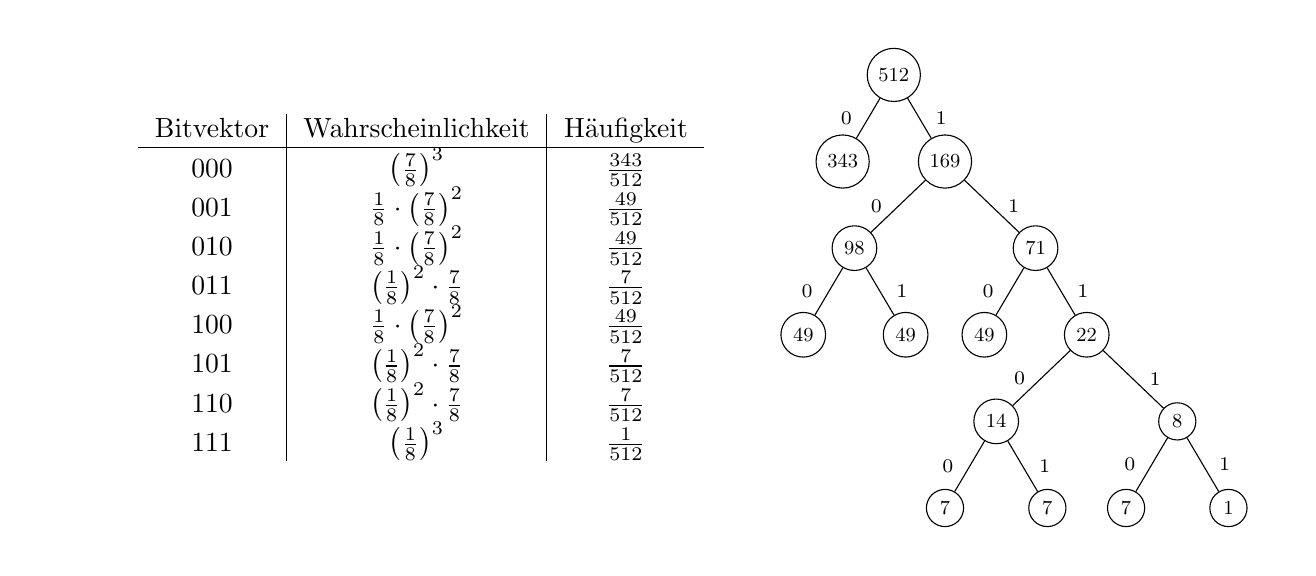
\begin{tikzpicture}[font=\small,every node/.style={shape=circle},
					    level 1/.style={sibling distance=1.3cm,level distance=1.1cm},
					    level 2/.style={sibling distance=2.3cm},
					    level 3/.style={sibling distance=1.3cm},
					    level 4/.style={sibling distance=2.3cm},
					    level 5/.style={sibling distance=1.3cm}]
				\path[use as bounding box] (-5,-3.3) rectangle (11,3.3);
				\node[scale=1.0,font=\normalsize] (tbl) {
				\begin{tabular}{c|c|c}
				        Bitvektor & Wahrscheinlichkeit & Häufigkeit \\
				        \hline
				        000& $\left(\frac{7}{8}\right)^3$ & $\frac{343}{512}$ \\
				        001& $\frac{1}{8}\cdot\left(\frac{7}{8}\right)^2$ & $\frac{49}{512}$ \\
				        010& $\frac{1}{8}\cdot\left(\frac{7}{8}\right)^2$ & $\frac{49}{512}$ \\
				        011& $\left(\frac{1}{8}\right)^2\cdot\frac{7}{8}$ & $\frac{7}{512}$ \\
				        100& $\frac{1}{8}\cdot\left(\frac{7}{8}\right)^2$ & $\frac{49}{512}$ \\
				        101& $\left(\frac{1}{8}\right)^2\cdot\frac{7}{8}$ & $\frac{7}{512}$ \\
				        110& $\left(\frac{1}{8}\right)^2\cdot\frac{7}{8}$ & $\frac{7}{512}$ \\
				        111& $\left(\frac{1}{8}\right)^3$ & $\frac{1}{512}$
				\end{tabular}};
				\node[scale=0.8,draw] at (6,2.7) {512}
				  child {
				    node[scale=0.8,draw] {343}
				    edge from parent
				    node[font=\scriptsize,left] {0}
				  }
				  child {
				    node[scale=0.8,draw] {169}
				      child {
				        node[scale=0.8,draw] {98}
					  child {
					    node[scale=0.8,draw] {49}
					    edge from parent
					    node[font=\scriptsize,left] {0}
					  }
					  child {
					    node[scale=0.8,draw] {49}
					    edge from parent
					    node[font=\scriptsize,right] {1}
					  }
					  edge from parent
					  node[font=\scriptsize,left] {0}
				      }
				      child {
				        node[scale=0.8,draw] {71}
					  child {
					    node[scale=0.8,draw] {49}
					    edge from parent
					    node[font=\scriptsize,left] {0}
					  }
					  child {
					    node[scale=0.8,draw] {22}
					      child {
					        node[scale=0.8,draw] {14}
						  child {
						    node[scale=0.8,draw] {7}
						    edge from parent
						    node[font=\scriptsize,left] {0}
						  }
						  child {
						    node[scale=0.8,draw] {7}
						    edge from parent
						    node[font=\scriptsize,right] {1}
						  }
						  edge from parent
						  node[font=\scriptsize,left] {0}
					      }
					      child {
					        node[scale=0.8,draw] {8}
						  child {
						    node[scale=0.8,draw] {7}
						    edge from parent
						    node[font=\scriptsize,left] {0}
						  }
						  child {
						    node[scale=0.8,draw] {1}
						    edge from parent
						    node[font=\scriptsize,right] {1}
						  }
						  edge from parent
						  node[font=\scriptsize,right] {1}
					      }
					      edge from parent
					      node[font=\scriptsize,right] {1}
					  }
					  edge from parent
					  node[font=\scriptsize,right] {1}
				      }
				    edge from parent
				    node[font=\scriptsize,right] {1}
				  };
			\end{tikzpicture}
			\end{table}
			
			Die mittlere Wortlänge ist $\mu_{1/8}^{(3)} =
			\frac{1}{512} \left(343\cdot1 + 49\cdot3\cdot3 +
			7\cdot5\cdot3 + 1\cdot5\right) \approx 1.75$.

		\item Nach dem Quellcodierungstheorem von \textsc{Shannon} gilt
			für die mittlere Höhe des Baumes $t$ mit
			Wahrscheinlichkeitsverteilung
			$\beta_p^{(n)}$
			\[
			  \operatorname{H}\left(\beta_p^{(n)}\right) \leq
			  h\left(t, \beta_p^{(n)}\right) \leq
			  \operatorname{H}\left(\beta_p^{(n)}\right) + 1.
			\]
			Die mittlere Codelänge $\mu_p^{(n)}$ ist genau
			$h\left(t, \beta_p^{(n)}\right)$. Mit
			$\operatorname{H}\left(\beta_p^{(n)}\right) = n \cdot
			\operatorname{H}(p, 1-p)$ ergibt sich nach Division
			durch $n$
			\[
			  \operatorname{H}(p, 1-p) \leq \frac{\mu_p^{(n)}}{n}
			  \leq \operatorname{H}(p, 1-p) + \frac{1}{n}.
			\]
			Die Grenzwerte für $n \rightarrow \infty$ der linken
			und rechten Seite der Ungleichung existieren und sind
			identisch, daher kann
			\[
			  \lim_{n\rightarrow\infty} \frac{\mu_p^{(n)}}{n} =
			  \operatorname{H}(p, 1-p)
			\]
			gefolgert werden.
		\end{flushalpha}
\end{flushenum}
